\chapter{Verteilte Anwendungen mit Sockets}

Eigenständige \codebf{Client-Server-Anwendungen} können auf 3 verschiedene Arten umgesetzt werden:

\begin{itemize}
    \item Socket-Programmierung (Socket: Schnittstelle für \textbf{UDP} / \textbf{TCP} \footnote{
    UDP: \textit{User Datagram Protocol}; TCP: \textit{Transmission Control Protocol}
    })
    \item \textbf{RMI} \textit{Remote Method Invocation}: Die Methode eines Objektes, das auf einem anderen Rechner liegt, kann von einem anderen entfernten Rechner aufgerufen werden; RMI basiert auf Sockets und stellt somit eine höhere Schnittstelle mit einem höheren Abstraktionsniveau dar
    \item \textbf{indirekte Kommunikation}: Nachrichten werden durch einen Vermittler von einem Sender zu einem Empfänger weitergeleitet
\end{itemize}


\subsection{Schichtenmodell}


\subsection*{Schicht 1 - (Physical Layer)}

Diese Schicht ist zuständig für die Übertragung von Datenblöcken zwischen zwei Rechnern, die direkt miteinander verbunden sind (genauso wie \textbf{Schicht 2}).\\
Sie ist zuständig für die Übertragung einzelner Bits und wird deshalb auch \textbx{Bitübertragungsschicht} genannt.

\subsection*{Schicht 2 - DataLink Layer}

Wie Schicht 1 ist auch diese Schicht zuständig für die Übertragung von Datenblöcken zwischen zwei direkt miteinander verbundenen Rechnern.\\

Die Schicht hat die Aufgabe, einzelne Bits zu einem Datenblock in einem bestimmten Format zusammenzufassen.\\
$\rightarrow$ bestimmte Informationen wie z.B. Adressen haben eine bestimmte Struktur und Bitlänge und stehen an bestimmten Stellen in einem Datenblock.\\

\noindent
Bei lokalen Netzen wie {bspw.} Ethernet hat die Leitungsschicht kommen durch das gemeinsame Medium noch weitere Funktionen: Sie garantiert, dass immer nur höchstens eine Station sendet, außerdem werden durch sie die angeschlossenen Rechner korrekt adressiert.

\begin{tcolorbox}
    Schicht 1 und 2 werden über Hardware ({bspw.} Ethernet-Adapter) und entsprechende Treiber im Betriebssystem realisiert.
\end{tcolorbox}

\noindent
Die beiden Funktionen (eine Station sendet, korrekte Adressierung) werden als \textbf{Medium Access Control} (\textit{MAC}) bezeichnet und bilden eine Teilschicht innerhalb der Leitungsschicht (\textit{DataLink Layer}).\\
Die entsprechenden Adressen heissen deshalb \textit{MAC-Adresssen}.

\subsection*{Schicht 3}
Schicht 3 ist die \textbf{Vermittlungsschicht} (\textbf{Network Layer}), hier befindet sich das \textbf{IP-Protokoll}, über das Rechner verbunden werden, die an verschiedene Netze mit unterschiedlichen Netztechnologien angeschlossen sind.\\

\noindent
Jeder Netzanschluss enthält eine eindeutige \textbf{IP-Adresse}.\\

\noindent
Über das IP-Protokoll werden Datenpakete über verschiedene Netze weitergeleitet, bis sie beim Zielrechner ankommen.\\

\noindent
Es kann durchaus vorkommen, dass Datenpakete verlorengehen, oder verzögert und/oder in unterschiedlicher Reihenfolge beim Empfänger eintreffen.


\begin{tcolorbox}
    Schicht 3 und 4 sind i.d.R. Teil des Betriebssystemkerns.
\end{tcolorbox}

\subsection*{Schicht 4}
Schicht 4 ergänzt die Adressierung in Schicht 3 um \textit{Konktaktpunkte} durch \textbf{Portnummern}, und wird \textbf{Transportschicht} (\textbf{Transport Layer}) genannt.\\

\noindent
Zwei verbreitete Transportprotokolle sind \textbf{UDP} und \textbf{TCP};

\begin{itemize}
    \item \textbf{UDP} (\textit{User Datagram Protocol}) hat dieselbe Eigenschaften wie das IP-Protokoll und erweitert es um die Adressierung mit Portnummern.\\
    Es ist genauso verbindungslos und unzuverlässig wie das IP-Protokoll.
    \item \textbf{TCP} (\textit{Transmission Control Protocol}) behebt die Nachteile des IP-Protokolls: Die Empfänger müssen den Nachrichtenerhalt bestätigen, ansonsten wird die Nachricht nochmals gesendet.
\end{itemize}


\subsection*{Schicht 5}
Schicht 5 ist die \textbf{Anwendungsschicht} (\textbf{Application Layer}), in ihr wird die Kommunikation der Anwendung abgewickelt (bspw. \textit{www}, \textit{email}, \textit{Videokonferenzen}).


\begin{tcolorbox}
    Schicht 5 wird über Anwendungsprozesse realisiert.
\end{tcolorbox}


\begin{figure}
    \centering
    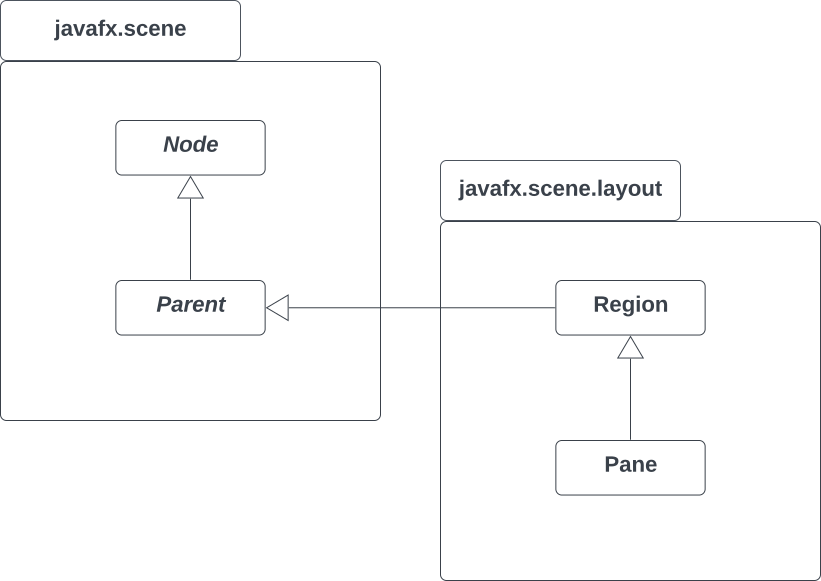
\includegraphics[scale=0.5]{chapters/fopt3/img/javafx/pane}
    \caption{Skizze des Schichtenmodels. (Quelle: in Anlehnung an \cite[257, Bild 5.2]{Oec22})}
    \label{fig:layers}
\end{figure}
